% mnras_template.tex 
%
% LaTeX template for creating an MNRAS paper
%
% v3.0 released 14 May 2015
% (version numbers match those of mnras.cls)
%
% Copyright (C) Royal Astronomical Society 2015
% Authors:
% Keith T. Smith (Royal Astronomical Society)

% Change log
%
% v3.0 May 2015
%    Renamed to match the new package name
%    Version number matches mnras.cls
%    A few minor tweaks to wording
% v1.0 September 2013
%    Beta testing only - never publicly released
%    First version: a simple (ish) template for creating an MNRAS paper

%%%%%%%%%%%%%%%%%%%%%%%%%%%%%%%%%%%%%%%%%%%%%%%%%%
% Basic setup. Most papers should leave these options alone.
\documentclass[fleqn,usenatbib]{mnras}

% MNRAS is set in Times font. If you don't have this installed (most LaTeX
% installations will be fine) or prefer the old Computer Modern fonts, comment
% out the following line
\usepackage{newtxtext,newtxmath}
% Depending on your LaTeX fonts installation, you might get better results with one of these:
%\usepackage{mathptmx}
%\usepackage{txfonts}

% Use vector fonts, so it zooms properly in on-screen viewing software
% Don't change these lines unless you know what you are doing
\usepackage[T1]{fontenc}
\usepackage{ae,aecompl}


%%%%% AUTHORS - PLACE YOUR OWN PACKAGES HERE %%%%%
% Only include extra packages if you really need them. Common packages are:
\usepackage{graphicx}	% Including figure files
\usepackage{amsmath}	% Advanced maths commands
\usepackage{amssymb}	% Extra maths symbols
\let\plate\undefined
\usepackage{tikz}
\usetikzlibrary{bayesnet}

%%%%%%%%%%%%%%%%%%%%%%%%%%%%%%%%%%%%%%%%%%%%%%%%%%

%%%%% AUTHORS - PLACE YOUR OWN COMMANDS HERE %%%%%

\newcommand{\aw}[1]{\textcolor{red}{[AW: #1]}}
\newcommand{\hvp}[1]{\textcolor{green}{[HVP: #1]}}
\newcommand{\dm}[1]{\textcolor{magenta}{[DM: #1]}}


\newcommand{\popp}{\boldsymbol{\Psi}}
\newcommand{\objp}{\boldsymbol{\psi}}
\newcommand{\data}{\mathbf{d}}
\newcommand{\Teff}{T}
\newcommand{\logg}{g}
\newcommand{\pr}{\text{Pr}}
\newcommand{\de}{\text{d}}
\newcommand{\kpc}{\text{kpc}}
\newcommand{\K}{\text{K}}


% Please keep new commands to a minimum, and use \newcommand not \def to avoid
% overwriting existing commands. Example:
%\newcommand{\pcm}{\,cm$^{-2}$}	% per cm-squared

%%%%%%%%%%%%%%%%%%%%%%%%%%%%%%%%%%%%%%%%%%%%%%%%%%

%%%%%%%%%%%%%%%%%%% TITLE PAGE %%%%%%%%%%%%%%%%%%%

% Title of the paper, and the short title which is used in the headers.
% Keep the title short and informative.
\title[Inferring properties of the white dwarf population]{Inferring properties of the local white dwarf population in astrometric and photometric surveys}

% The list of authors, and the short list which is used in the headers.
% If you need two or more lines of authors, add an extra line using \newauthor
\author[A. Widmark et al.]{
Axel Widmark,$^1$\thanks{E-mail: axel.widmark@fysik.su.se} 
D. Mortlock,$^{1,2}$
H. Peiris$^{1,3}$
\\
% List of institutions
$^1$The Oskar Klein Centre for Cosmoparticle Physics, Department of
Physics, Stockholm University, AlbaNova, 10691 Stockholm, Sweden\\
$^2$Imperial\\
$^3$UCL\\
}

% These dates will be filled out by the publisher
\date{Accepted XXX. Received YYY; in original form ZZZ}

% Enter the current year, for the copyright statements etc.
\pubyear{2018}

% Don't change these lines
\begin{document}
\label{firstpage}
\pagerange{\pageref{firstpage}--\pageref{lastpage}}
\maketitle

% Abstract of the paper
\begin{abstract}
The Gaia mission will provide precise astrometry for an unprecedented number of white dwarfs (WDs), promising enormous scientific potential. With such a large data set, it is possible to infer properties of the WD population using only astrometric and photometric information. We demonstrate a framework to accomplish this using a mock data set with SDSS \emph{ugriz} photometry and astrometric information expected from future Gaia data releases.
Our technique utilises a Bayesian hierarchical model, a powerful tool for inferring properties of a stellar population while also taking into account all observational errors of individual stars. We demonstrate that astrometry significantly improves the statistical inference, leading to more robust conclusions which are less sensitive to systematic errors.
This is a powerful method for constraining stellar evolution, especially Type 1a supernovae progenitor scenarios, as well as the star formation and dynamical history of the Milky Way.
\end{abstract}

% Select between one and six entries from the list of approved keywords.
% Don't make up new ones.
\begin{keywords}
white dwarfs -- stars: statistics -- astrometry
\end{keywords}

%%%%%%%%%%%%%%%%%%%%%%%%%%%%%%%%%%%%%%%%%%%%%%%%%%

%%%%%%%%%%%%%%%%% BODY OF PAPER %%%%%%%%%%%%%%%%%%







\section{Introduction}

White dwarfs (WDs) are the eventual remnants of all light to intermediate mass stars. The WD population carries information about the Galaxys's star formation history and dynamical history and constrain models of stellar evolution. WDs are known to be SN1A thermonuclear supernovae progenitors, although the explosion mechanism is poorly understood.

The Sloan Digital Sky Survey (SDSS) catalogues a total number of $\sim 29,000$ spectroscopically confirmed white dwarfs \citep{2013ApJS..204....5K,2015MNRAS.446.4078K}. A fundamental difficulty in studying white dwarfs (WDs) is that they have no fixed mass or size, such that their observational properties are largely degenerate with distance. This degeneracy can be broken with high quality spectrometry and accurate atmospheric models, although this is sensitive to systematic errors. The Gaia mission, soon to publish its second data release (DR2), is expected to increase the number of known white dwarfs by something like an order of magnitude \citep{2014A&A...565A..11C,Jordan:2006jg}. Gaia will also provide astrometric information for local neighbourhood white dwarfs, which previous astrometric missions were unable to do. Hipparcos had a limiting apparent magnitude of $V \sim 12.4$, while Gaia will see objects as dim as $G \sim 21$.

With the enormous size of the Gaia data set, there is great potential in an approach that focuses on width rather than depth, by taking less detailed information into account but including a very large number of objects. In this article we demonstrate how to infer properties of the white dwarf population in the solar neighborhood, using SDSS \emph{ugriz} photometry and Gaia astrometry. We generate a mock data sample of white dwarfs from a population model of temperature, surface gravity and spatial number density distributions. All sample objects has photometry and parallax information with observational errors expected from SDSS and Gaia, and sample construction selection effects are taken into account. We retain the parameters of the population model using a Bayesian hierarchical model, which is a powerful tool to infer properties of a stellar population while also taking into account all observational errors of individual stars.

White dwarfs form a family of phenomenological types, where the main classification is between DA and DB, depending on if the envelope is hydrogen or helium dominated. DA and DB stars can be identified with accurate photometry, as demonstrated by \cite{Mortlock:2008gf}. We demonstrate that we are able to infer the relative stellar number ratio of DA and DB systems. We also discuss how to expand the statistical model when considering other WD sub--populations. We consider separate disk and halo WD populations, which are expected to have different properties. The halo population is older, and holds information about the Milky Way's distant past. We also discuss the possibility of identifying binary WD systems using this method, which can be done using photometric and astrometric information alone.

This paper is organized as follows...





\section{Model}\label{sec:model}

In this section we describe a model for the Milky Way white dwarf population. This population model includes the white dwarf spatial distribution, as well as distributions in intrinsic white dwarf properties, parameterized by effective temperature, surface gravity, and type.

We list the population parameters of our model, encapsulated in a vector $\popp$, in table \ref{tab:parameters}, along with the object parameters and data. The population parameters are $\alpha$, which parameterizing the distribution of temperatures, and $\bar{g}$, $\sigma_g$, $\gamma_g$ which parameterize the distribution of surface gravities.

The distribution of surface gravity and effective temperature are parameterized by

\begin{equation}\label{eq:T&g}
\begin{split}
	\pr(\logg | \popp) & \propto \Theta(\logg \in [7,9]) \times f_t(\logg|\bar{g},\sigma_g,\gamma_g),\\
    \pr(\Teff | \popp) & \propto \Theta(\Teff/\K \in [1500,120000]) \times \exp (-\alpha \Teff),
\end{split}
\end{equation}
where $\Theta$ is a step function, $f_t(\logg)$ is the Student's t-distribution of width $\sigma_g$ and variance $\text{Var}(g) = \gamma_g^2 \sigma_g^2$, such that the quantity $\gamma_g$ parameterizes the heaviness of the distribution's tails. The surface gravity $\logg$ is limited to the interval $[7,9]$.

The class of the object constitutes a third parameter of the intrinsic white dwarf properties, called $t$. This is not continuous but a label, denoting for example if the white dwarf is of DA or DB classification. The probabilities are written in terms of population parameter $f_\text{DB}$, which is the fraction of DB WDs, like
\begin{equation}\label{eq:DADB}
\begin{split}
	\pr(t=\text{DA} | \popp) & = (1-f_\text{DB}),\\
    \pr(t=\text{DB} | \popp) & = f_\text{DB}.
\end{split}
\end{equation}

Given the intrinsic properties of a white dwarf, the absolute magnitude in different photometric bands can be calculated using a stellar model. In this paper, we use the Bergeron atmospheric model for white dwarfs \citep{Bergeron:1995we,Finley:1997zz,Bergeron:2000ce,2001PASP..113..409F}.

Also included in our model is a white dwarf number density function, expressed in terms of cylindrical coordinates $R$, $Z$ and $\Phi$,

\begin{equation}\label{eq:numberdensity}
\begin{split}
	n(\mathbf{x}) \propto
	\Bigg[ 
		& \exp\Bigg(-\frac{R}{L_\text{thin}}\Bigg)\exp\Bigg(-\frac{|Z|}{H_\text{thin}}\Bigg) \\
		& +f_\text{thick}\exp\Bigg(-\frac{R}{L_\text{thick}}\Bigg)\exp\Bigg(-\frac{|Z|}{H_\text{thick}}\Bigg) \\
		& +f_\text{halo}\Bigg( \frac{(R^2+Z^2/q_\text{halo}^2+R_\text{core}^2)^{1/2}}{L_\text{halo}}^{-\eta_\text{halo}} \Bigg),
	\Bigg]
\end{split}
\end{equation}
where $f_\text{thick}=0.06$, $f_\text{halo}=6\times10^{-5}$, $L_\text{thin}=L_\text{thick}=3.5~\kpc$, $L_\text{halo}=8.5~\kpc$, $R_\text{core}=1~\kpc$, $H_\text{thin}=0.26~\kpc$, $H_\text{thick}=1~\kpc$, $q_\text{halo}=0.64$ and $\eta_\text{halo} = 2$. Assuming a solar position of $R_\odot=8~\kpc$ (where the height of the Sun above the plane is neglected), the galactic coordinates are given by heliocentric coordinates through

\begin{equation}
\begin{split}
	& R(d,l,b) = [d^2\cos^2b-2 R_\odot d \cos^2b\cos^2+R_\odot^2]^{1/2}, \\
	& Z(d,l,b) = d \sin b.
\end{split}
\end{equation}
The azimuthal angle can be neglected, as the galaxy is assumed to be axisymmetric in this model.



\begin{table}
	\centering
	\caption{The population parameters of our model, and the object parameters and data of the respective stars.}
	\label{tab:parameters}
    \begin{tabular}{l l}
		\hline
		$\popp$  & Population parameters \\
		\hline
		$\alpha$ & -- slope of temperature distribution \\
		$\bar{g}$ & -- mean and median surface gravity $\logg$ \\
		$\sigma_g$ & -- width of $\logg$ distribution \\
		$\gamma_g$ & -- heavieness of the tails of the $\logg$ distribution \\
		$f_\text{DB}$ & -- the fraction of DB type WDs \\
        \hline
        $\objp_{i=1,...,n}$  & Object parameters \\
        \hline
        $\Teff$ & -- effective temperature \\
        $\logg$ & -- surface gravity \\
        $t$ & -- WD classification (DA or DB) \\
        $\mathbf{x}$ & -- spatial position  \\
        \hline
        $\data_{i=1,...,n}$ & Data \\
        \hline
        $\hat{m}_b$,& -- observed photometric magnitude \\
        $\sigma_b$ & -- magnitude uncertainty \\
        $\hat{\varpi}$ & -- observed parallax \\
        $\sigma_{\hat{\varpi}}$ & -- parallax uncertainty \\
        $l$ & -- observed galactic longitude \\
        $b$ & -- observed galactic latitude \\
		\hline
	\end{tabular}
\end{table}




\section{Data}\label{sec:data}

We will demonstrate how to infer properties of a white dwarf population given photometric and astrometric data. We begin by discussing the general case and how to construct a likelihood for the properties of a white dwarf. We then discuss the specific case of combining SDSS photometry and Gaia astrometry, and what errors are expected for the two surveys.

The data of a white dwarf consists of apparent magnitude in some number of photometric bands ($\hat{m}_b$), a parallax measurement ($\hat{\varpi}$), angular position ($l$ and $b$), and errors on these observables. A hatted quantity ($\hat{\varpi}$) refers to an observed value of some measurement error, while a non-hatted quantity ($\varpi$) refers to an observable's true value. The angles $l$ and $b$ are written without hats, to signify that they are taken at face values, as the errors are small and can be neglected. The data of a white dwarf with index $i$, called $\data_i$, is listed in Table \ref{tab:parameters}.

The likelihood of a white dwarf, denoted by an index $i$, is written

\begin{equation}\label{eq:likelihood}
	\pr(\data_i | \objp_i) = \mathcal{N}(\varpi(\objp_i)|\hat{\varpi},\sigma_{\hat{\varpi}})\prod_{b} \mathcal{N}(m_b(\objp_i)|\hat{m}_b,\sigma_b),
\end{equation}
where the color bands are iterated over in the product, and $\mathcal{N}(x | \mu,\sigma)$ is the normal distribution of mean $\mu$ and standard deviation $\sigma$. The factor containing parallax information is dropped when no parallax information is present. The apparent magnitudes $m_b(\objp_i)$ are functions of the object parameters, coming from a stellar model.

In this article, we use SDSS photometry in \emph{ugriz} color bands, and a Bergeron atmospheric stellar model, as discussed in Sec. \ref{sec:model}. In order to assign realistic errors to the mock data that we generate, we use median errors of the SDSS DR9 catalogue, in bins of observed apparent magnitude of width 0.5 mag. These median errors are visible in Fig. \ref{fig:magnitude_error}. We limit the minimum \emph{ugriz} magnitude error to 0.01, in order to account for possible systematic errors.

\begin{figure}
	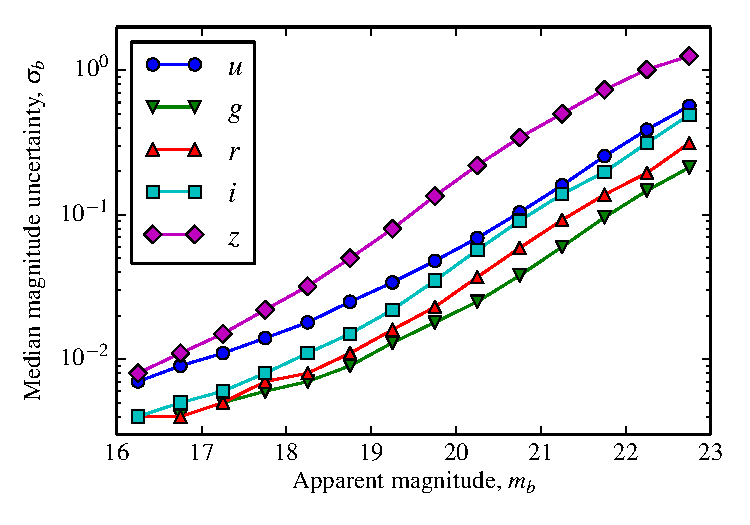
\includegraphics[width=\columnwidth]{median_app_errors.pdf}
    \caption{The median magnitude errors in SDSS DR9, as a function of observed apparent magnitude.}
    \label{fig:magnitude_error}
\end{figure}

We use parallax information with precision expected from Gaia DR2. DR2 will have a limiting magnitude of $G \simeq 21$, with parallax uncertainties smaller than $0.04$ mas for sources with $m_G<15$, about $0.1$ mas for sources with $m_G=17$, and about $0.7$ mas at $m_G=20$.\footnote{https://www.cosmos.esa.int/web/gaia/dr2} In order to account for this magnitude dependence, we interpolate these points according to Fig. \ref{fig:parallax_error}. The errors in the Gaia photometric $G$-band are interpolated in the same manner as for the parallax, with errors of 0.3 mmag for $m_G = 13$, 2 mmag for $m_G = 17$, and 10 mmag for $m_G = 20$.

\begin{figure}
	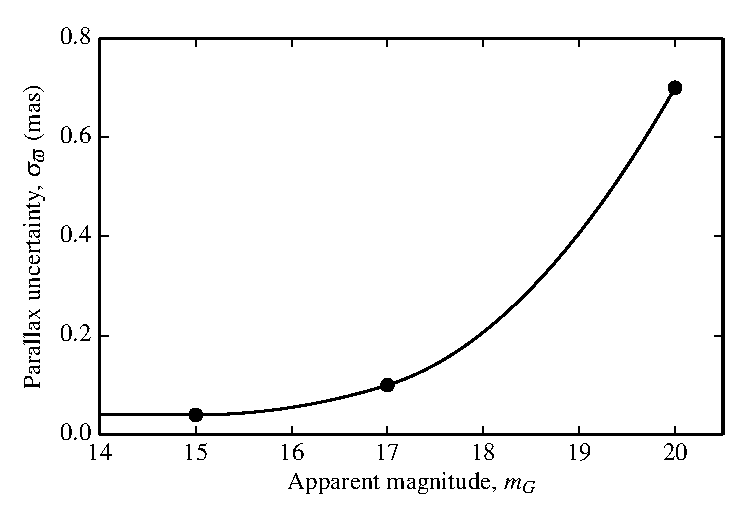
\includegraphics[width=\columnwidth]{parallax_error.pdf}
    \caption{Parallax error as a function of Gaia $G$--band apparent magnitude $m_G$. The dots correspond to magnitudes $m_G=\{15,17,20\}$. For $m_G\leq 15$ the parallax error is 0.04 mas and constant.}
    \label{fig:parallax_error}
\end{figure}





\section{Method}\label{sec:method}

The full posterior on both population parameters and object parameters is written

\begin{equation}\label{eq:fullposterior}
	\pr(\popp,\objp | \data ) = \pr(\popp)
    \prod_i \frac{S(\data_i) \pr(\data_i|\objp_i) \pr(\objp_i | \popp)}{\bar{N}(S,\popp)},
\end{equation}
where $\pr(\popp)$ is a prior on the population parameters; $S(\data_i)$ is the probability of being selected given the data of that object; $\pr(\data_i|\objp_i)$ is the likelihood of the data of an object given its object parameters; $\pr(\objp_i | \popp)$ is the probability of object parameters given the population parameters; finally, $\bar{N}(S,\popp)$ is the normalization to $\pr(\objp_i | \popp)$, and depends on the selection function and the population parameters. When writing the data or object parameters without an index $i$, we refer to the complete set of objects, $\objp \equiv \{ \objp_1,\objp_2,...,\objp_N \}$.

A directed acyclical graph (DAG) of our statistical model is visible in Fig.~\ref{fig:DAG}.

\begin{figure}\label{fig:DAG}
  \centering
  \tikz{
    \node[latent] (popp) {$\boldsymbol{\Psi}$} ; %
    \node[latent, below=of popp] (distfunc) {$F$} ; %
    \node[latent, left=of distfunc, rectangle] (selection) {$S$} ; %
    \node[latent, below=of distfunc] (objp) {$\boldsymbol{\psi}$} ; %
    \node[latent, left=of objp, rectangle] (data) {$\boldsymbol{d}$} ; %
    \plate[inner sep=0.3cm, xshift=-0.0cm, yshift=0.16cm] {index_i} {(data) (objp)} {i}; %
    \edge[dotted] {popp} {distfunc} ; %
    \edge[dotted] {selection} {distfunc} ; %
    \edge {distfunc} {objp} ; %
    \edge {data} {objp} ; %
  }
  \caption{A directed acyclical graph (DAG) of our statistical model. Quantities inscribed in circles (squares) represent variables (constants); solid (dotted) arrows represent probabilistic (deterministic) dependence; a rectangle with rounded corners represents a set of objects, in this case the set of WD included in our sample. The quantity $F$ is the normalized WD distribution function.}
\end{figure}







\subsection{Object parameters}\label{sec:objectparams}

Each white dwarf has a set of object parameters encapsulated in $\objp_i$, as listed in table \ref{tab:parameters}. It consists of the effective temperature $\Teff$, the surface gravity $\logg$, the type $t$ denoting DA or DB classification, and $\Delta$ which parameterizes the distance.

Conceptually, the most straight forward parameterization would be to have the distance $d$ as the third object parameter. However, this creates some sampling difficulties coming from the fact that $\logg$ and $d$ are heavily degenerate, which is problematic especially when there is no parallax information that constrains the distance. This is illustrated in Fig. \ref{fig:banana}. Therefore the distance is parameterized in terms of $\Delta$, which is the relative change to the ideal distance given $\Teff$ and $\logg$. Let $\tilde{d}(\Teff,\logg)$ be the distance that maximizes the color factor of the likelihood function, like

\begin{equation}
	\tilde{d} = 
    h^{-1}\left( \frac{\sum_b \sigma_b^{-2} (\hat{m}_c-M_c(\Teff,\logg))}{\sum_b \sigma_b^{-2}} \right),
\end{equation}
where $h^{-1}$ is the inverse of $h(d)=5[\log_{10}(d/\text{pc})-1]$, which is the difference between apparent to absolute magnitude. The distance parameterized by the object parameters is then $d=\Delta\tilde{d}(\Teff,\logg)$. It is crucial to account for the Jacobian factor that arises with this parameterization, which is $\de \Teff\, \de \logg\, \de d = \de \Teff\, \de \logg\, \de \Delta\, \tilde{d}(\Teff,\logg)$.

\begin{figure}
	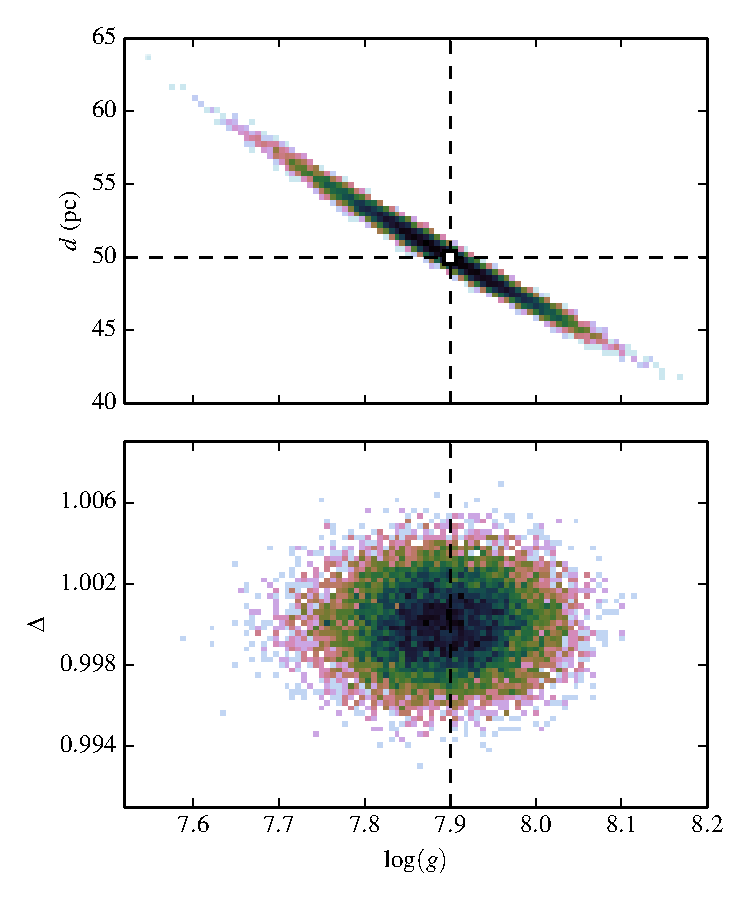
\includegraphics[width=\columnwidth]{banana.pdf}
    \caption{A posterior density of an object with true parameters $\Teff=20000$ K, $\logg=8$, $t=$DA, and $d=50$ pc, with photometric errors of $\sigma_c=0.03$ in all \emph{ugriz} color bands. The population parameters are set to $\alpha=3.5$, $\bar{g}=8$, $\sigma_g=0.1$, $\gamma_g=1.2$, and $f_\text{DB}=0$. Because the photometric errors are somewhat large, the constraint to the surface gravity is mostly due to the prior set by the population model. The top panel shows the posterior density over $\logg$ and $\Delta$, while the bottom panel shows the same posterior in a $\logg$ and $d$ parameterization. This illustrates the degeneracy between surface gravity $\logg$ and distance $d$, which can be problematic for a Metropolis-Hastings algorithm to sample.}
    \label{fig:banana}
\end{figure}







\subsection{Object posterior}\label{sec:objectposterior}

The posterior on a specific object also includes the term $\pr(\objp_i | \popp)$, normalized by the quantity $\bar{N}(S,\popp)$. It is given by the population, parameterized by the population parameters $\popp$,
\begin{equation}
\begin{split}
	& \pr(\objp_i | \popp)\, \de \Teff\, \de \logg\, \de d  \\ & \propto
    d^2 n(l,b,\varpi)\, \pr(\Teff,g,t | \popp)\, \de \Teff\, \de \logg\, \de d \\
    & = \Delta^2\, \tilde{d}^3(\Teff,\logg,t) n(l,b,\varpi)\, \pr(\Teff,g,t | \popp)\, \de \Teff\, \de\logg\, \de \Delta,
\end{split}
\end{equation}
where $n$ is the number density of white dwarfs as a function of spatial position (possible here to also include velocity, but will leave that for now). It is implicit in this expression that the true parallax $\varpi$ is a function of the object parameters $\objp_i$.

The normalization factor is given by an integral (or sum, in the case of a discrete variable) over the possible properties of a hypothetical white dwarf drawn from the population model, times the probability of being selected, like
\begin{equation}\label{eq:normalization}
	\bar{N}(S,\popp) = \sum_{t} \int \de\Teff\, \de \logg\, \de^3\mathbf{x}\,
    \pr(\Teff,g,t | \popp)\, n(\mathbf{x})\, S(\Teff,\logg,t,\mathbf{x}).
\end{equation}
The probability of being selected is the probability of being included in the sample, given by the cuts on observables and an object's intrinsic properties. This is formulated later in Sec.~\ref{sec:sample_cuts} and Eq.~\eqref{eq:selection}.



\section{Mock data and inference}\label{sec:mock}

To test the algorithm, mock data is generated from a population model, with population parameters $\alpha=3.5$, $\bar{g}=7.9$, $\sigma_g=0.1$, and $\gamma_g=1.2$, and the white dwarf number density $n(\mathbf{x})$ as described in section \ref{sec:model}. We compare the case of having no astrometric information, versus having parallax measurements with the precision expected from Gaia DR2.

\subsection{Sample cuts}\label{sec:sample_cuts}

We define a sample by making cuts on observable properties, either on actual data or in our case on mock data of a generated catalogue. Depending on the errors of these observables, these cuts correspond more or less well to cuts in the objects' intrinsic properties. In this case we make cuts on apparent magnitude and color. We do not make a volume limited sample by making cuts on parallax -- we want to compare to the case when astrometry is not available, hence we need to construct the sample without such information. The cuts in observed color is made such that we put upper and lower limits to the temperature of white dwarfs included in our sample. The limit in apparent magnitude sets a maximum distance for a white dwarf, as a function of temperature, where the hottest objects are seen to furthest distance.

There are several reasons for not allowing very high temperatures in our samples (although the exact limit is rather arbitrary). Very hot objects are rare, but because they are seen to much further distance they can still be numerous in a sample that is not volume limited. How many are seen depends on the properties of the population, but this is degenerate with the assumed spatial distribution and the distribution of dust. Furthermore, with high enough temperature the peak of an object's spectrum is of shorter wavelength than the $u$ band, in which case the inference on an objects temperature becomes very weak. When working with actual data, it is also necessary to identify what objects are white dwarfs and what objects are not. With a very hot, far away objects this is difficult, especially since the distance will be poorly constrained. These issues can be circumvented with good parallax measurements, enabling the construction of a volume limited sample.

We make the following cut in color, demanding that
\begin{equation}
	\hat{\delta}_{ugr} \equiv -0.4925\hat{m}_u-0.5075\hat{m}_g+\hat{m}_r \in (-0.6195,0.4369).
\end{equation}
Without measurement errors, this cut corresponds to limiting the temperature of a DA type WD to $\Teff \in (7000,30000)$ K; for a DB white dwarf the upper limit in temperature is less restrictive. This is illustrated in Fig. \ref{fig:colors_cut}.

\begin{figure}
	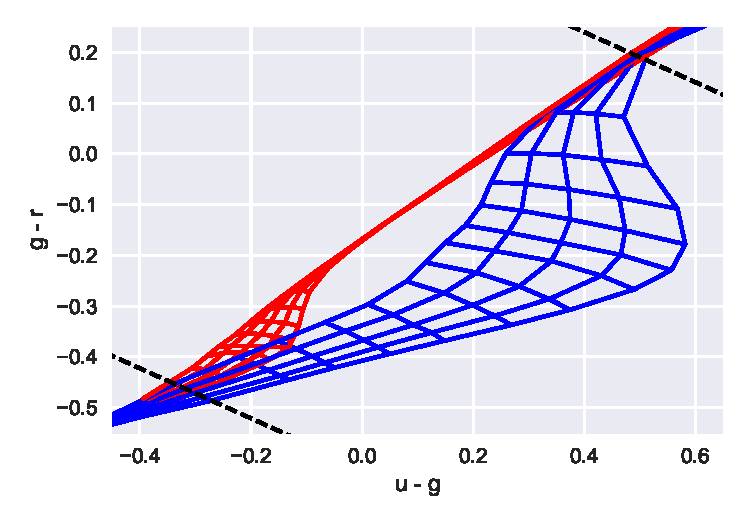
\includegraphics[width=\columnwidth]{colors_cut.pdf}
    \caption{Colors of a DA (blue grid) and DB (red grid) white dwarf, in lines of constant $\Teff$ or $\logg$. The surface gravity takes values $\logg = \{7,7.5,8,8.5,9\}$. The black dashed lines corresponds to the color cuts in $\hat{\delta}_{ugr}$, where only objects that fall in the region between these lines are included.}
    \label{fig:colors_cut}
\end{figure}

We also make a cut in brightness, by demanding that the Gaia $G$ band apparent magnitude fulfills that
\begin{equation}
	\hat{m}_G < 20.
\end{equation}
In principle, this criteria could equally well have been formulated in terms of some combination of the $ugriz$ apparent magnitudes.

Given these cuts to observables, the selection function is written
\begin{equation}\label{eq:selection}
\begin{split}
	S(\Teff,\logg,\mathbf{x}) = 
    	      \int \de \hat{m}_G \Theta \big( 20-\hat{m}_G \big)\mathcal{N}\big( \hat{m}_G | m_G,\sigma_{\hat{m}_G} \big) \\
    \times \int \de \hat{\delta}_{ugr} \Theta \big( \hat{\delta}_{ugr} \in (-0.6195,0.4369) \big) \mathcal{N}\big( \hat{\delta}_{ugr} | \delta_{ugr},\sigma_{\delta}\big),
\end{split}
\end{equation}
where the error on $\hat{\delta}_{ugr}$ is given by
\begin{equation}
	\sigma_\delta = \sqrt{ (0.4925 \sigma_u)^2 + (0.5075 \sigma_g)^2 + \sigma_r^2 },
\end{equation}
assuming that the different color band errors are uncorrelated.


\subsection{Generating a mock data catalogue}

The mock catalogue is generated by rejection sampling. An object is drawn randomly from the true population model: the object parameters $\Teff$ and $\logg$ are distributed as described in \eqref{eq:T&g} and can be randomized analytically; the position is distributed according to $n(\mathbf{x})$ and can be randomized by rejection sampling, knowing that there is a maximal distance a white dwarf can have to be included in our sample (observational errors included). A randomly drawn object is then given observable quantities with errors as described above. If the object observables fulfill the selection cuts, the object is included in the sample; if not, it is rejected.

In this article, we construct a sample with 10,000 WDs. The distribution of true parameter values is visible in Fig. \ref{fig:10000WDs}, where selection effects are manifest. The maximum distance is clearly seen as a function of temperature; due to the color cut, the high temperature tail is more pronounced for the DB sub--population. It is also clear that low mass WDs, which are more luminous, are more prone to being included in the sample, giving rise to some asymmetry in the distribution of surface gravity. The hottest object in this sample has an effective temperature of $\Teff=39,060$ K and is of DB class. The most distant object is located at 1.56 kpc and has an effective temperature $\Teff=37,287$ K surface gravity $\logg=7.72$ and is DA.

Our sample size of 10,000 DA white dwarfs is a reasonable number of white dwarfs given the cuts BLABLA

\begin{figure*}
	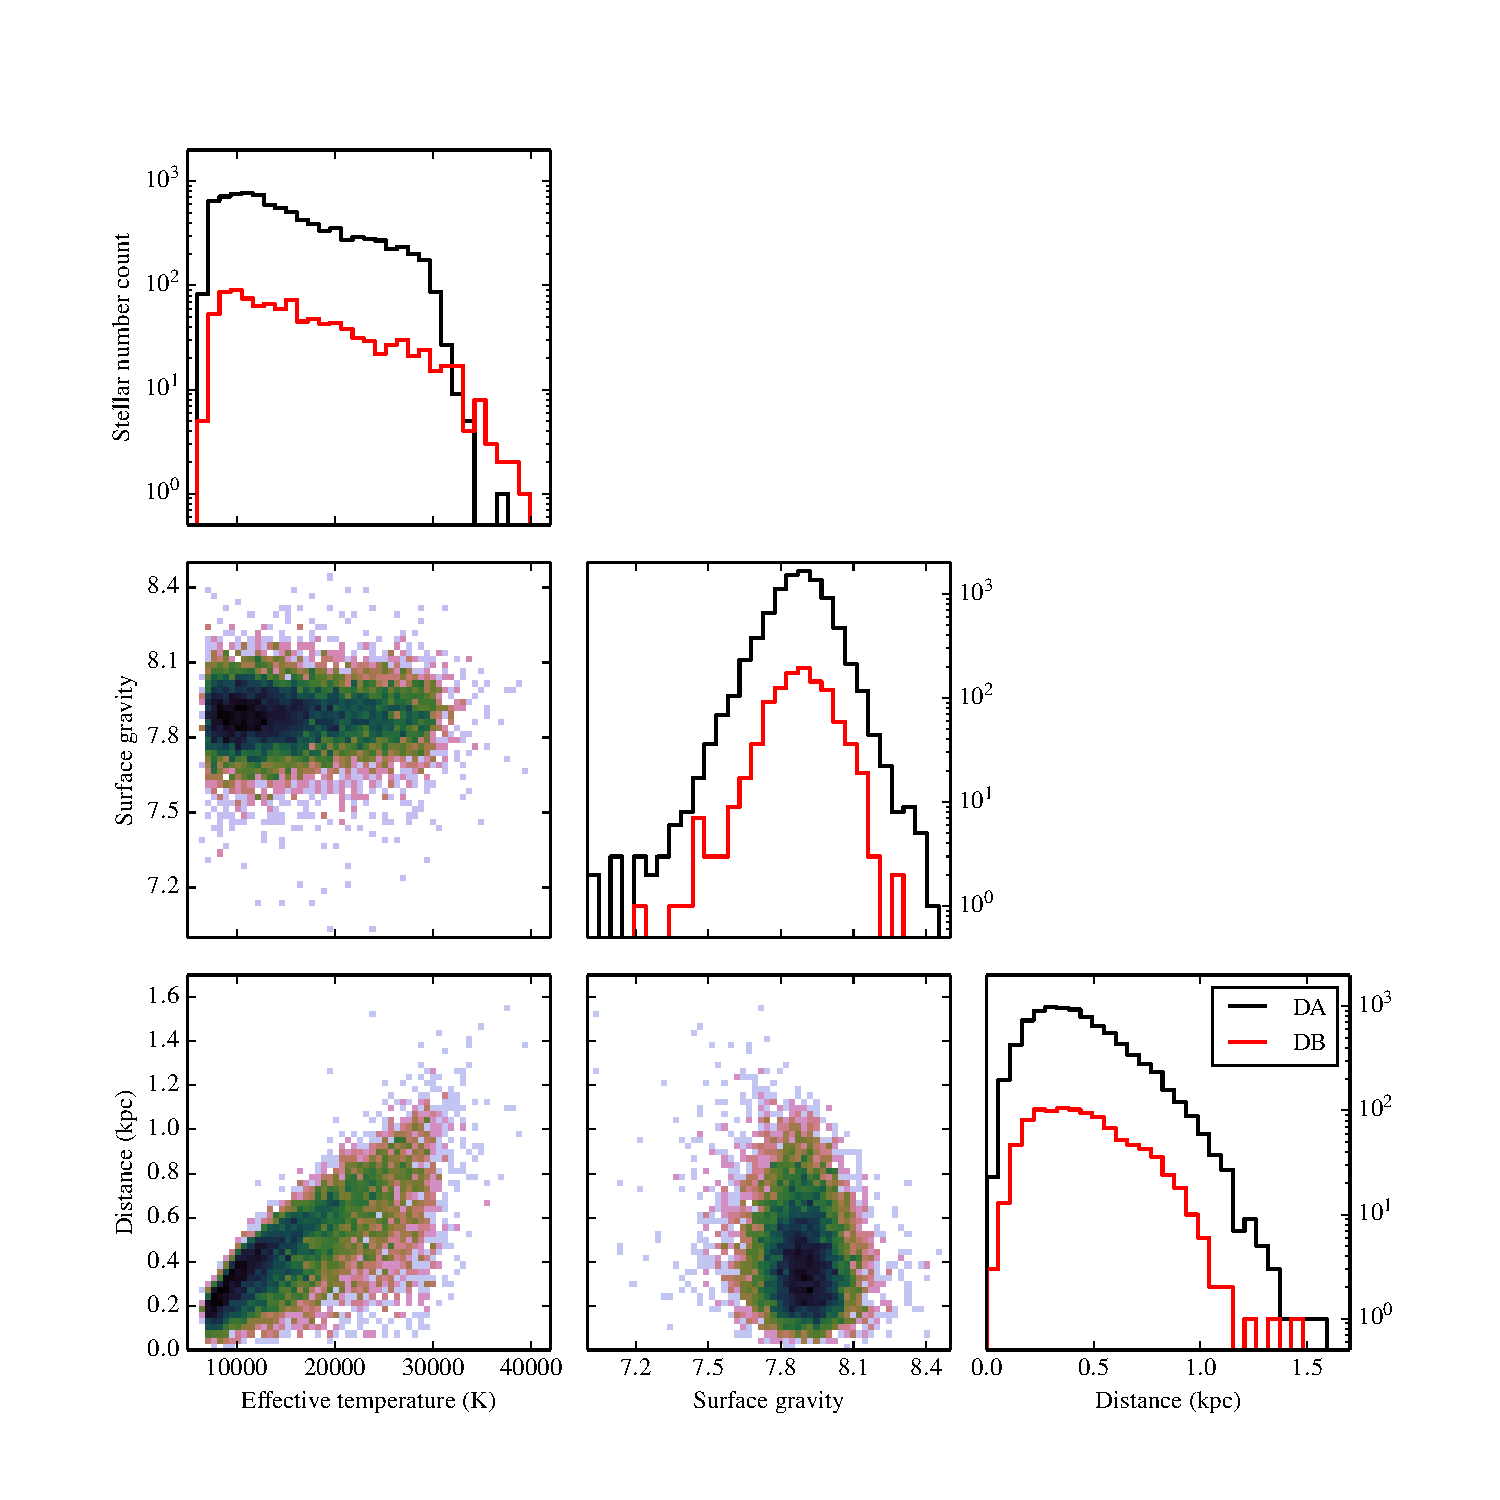
\includegraphics[width=.9\textwidth]{10000WDs.pdf}
    \caption{The distributions of true intrinsic properties of our mock data sample, represented as 1D and 2D histograms. The axis are shared between the figures, except for the vertical axis of the histograms. In the 2D histograms, there is no differentiation between DA and DB WDs. In the 1D histograms, the distribution of DA WDs are shown in blue, and DB WDs are shown in red.}
    \label{fig:10000WDs}
\end{figure*}



\subsection{Results}

RUN CHAIN WITH BURN-IN AND YADA YADA

The inferred posterior distributions are visible in Fig. \ref{fig:chain} and \ref{fig:chain_parallax}, where the former has no parallax information.

\begin{figure*}
	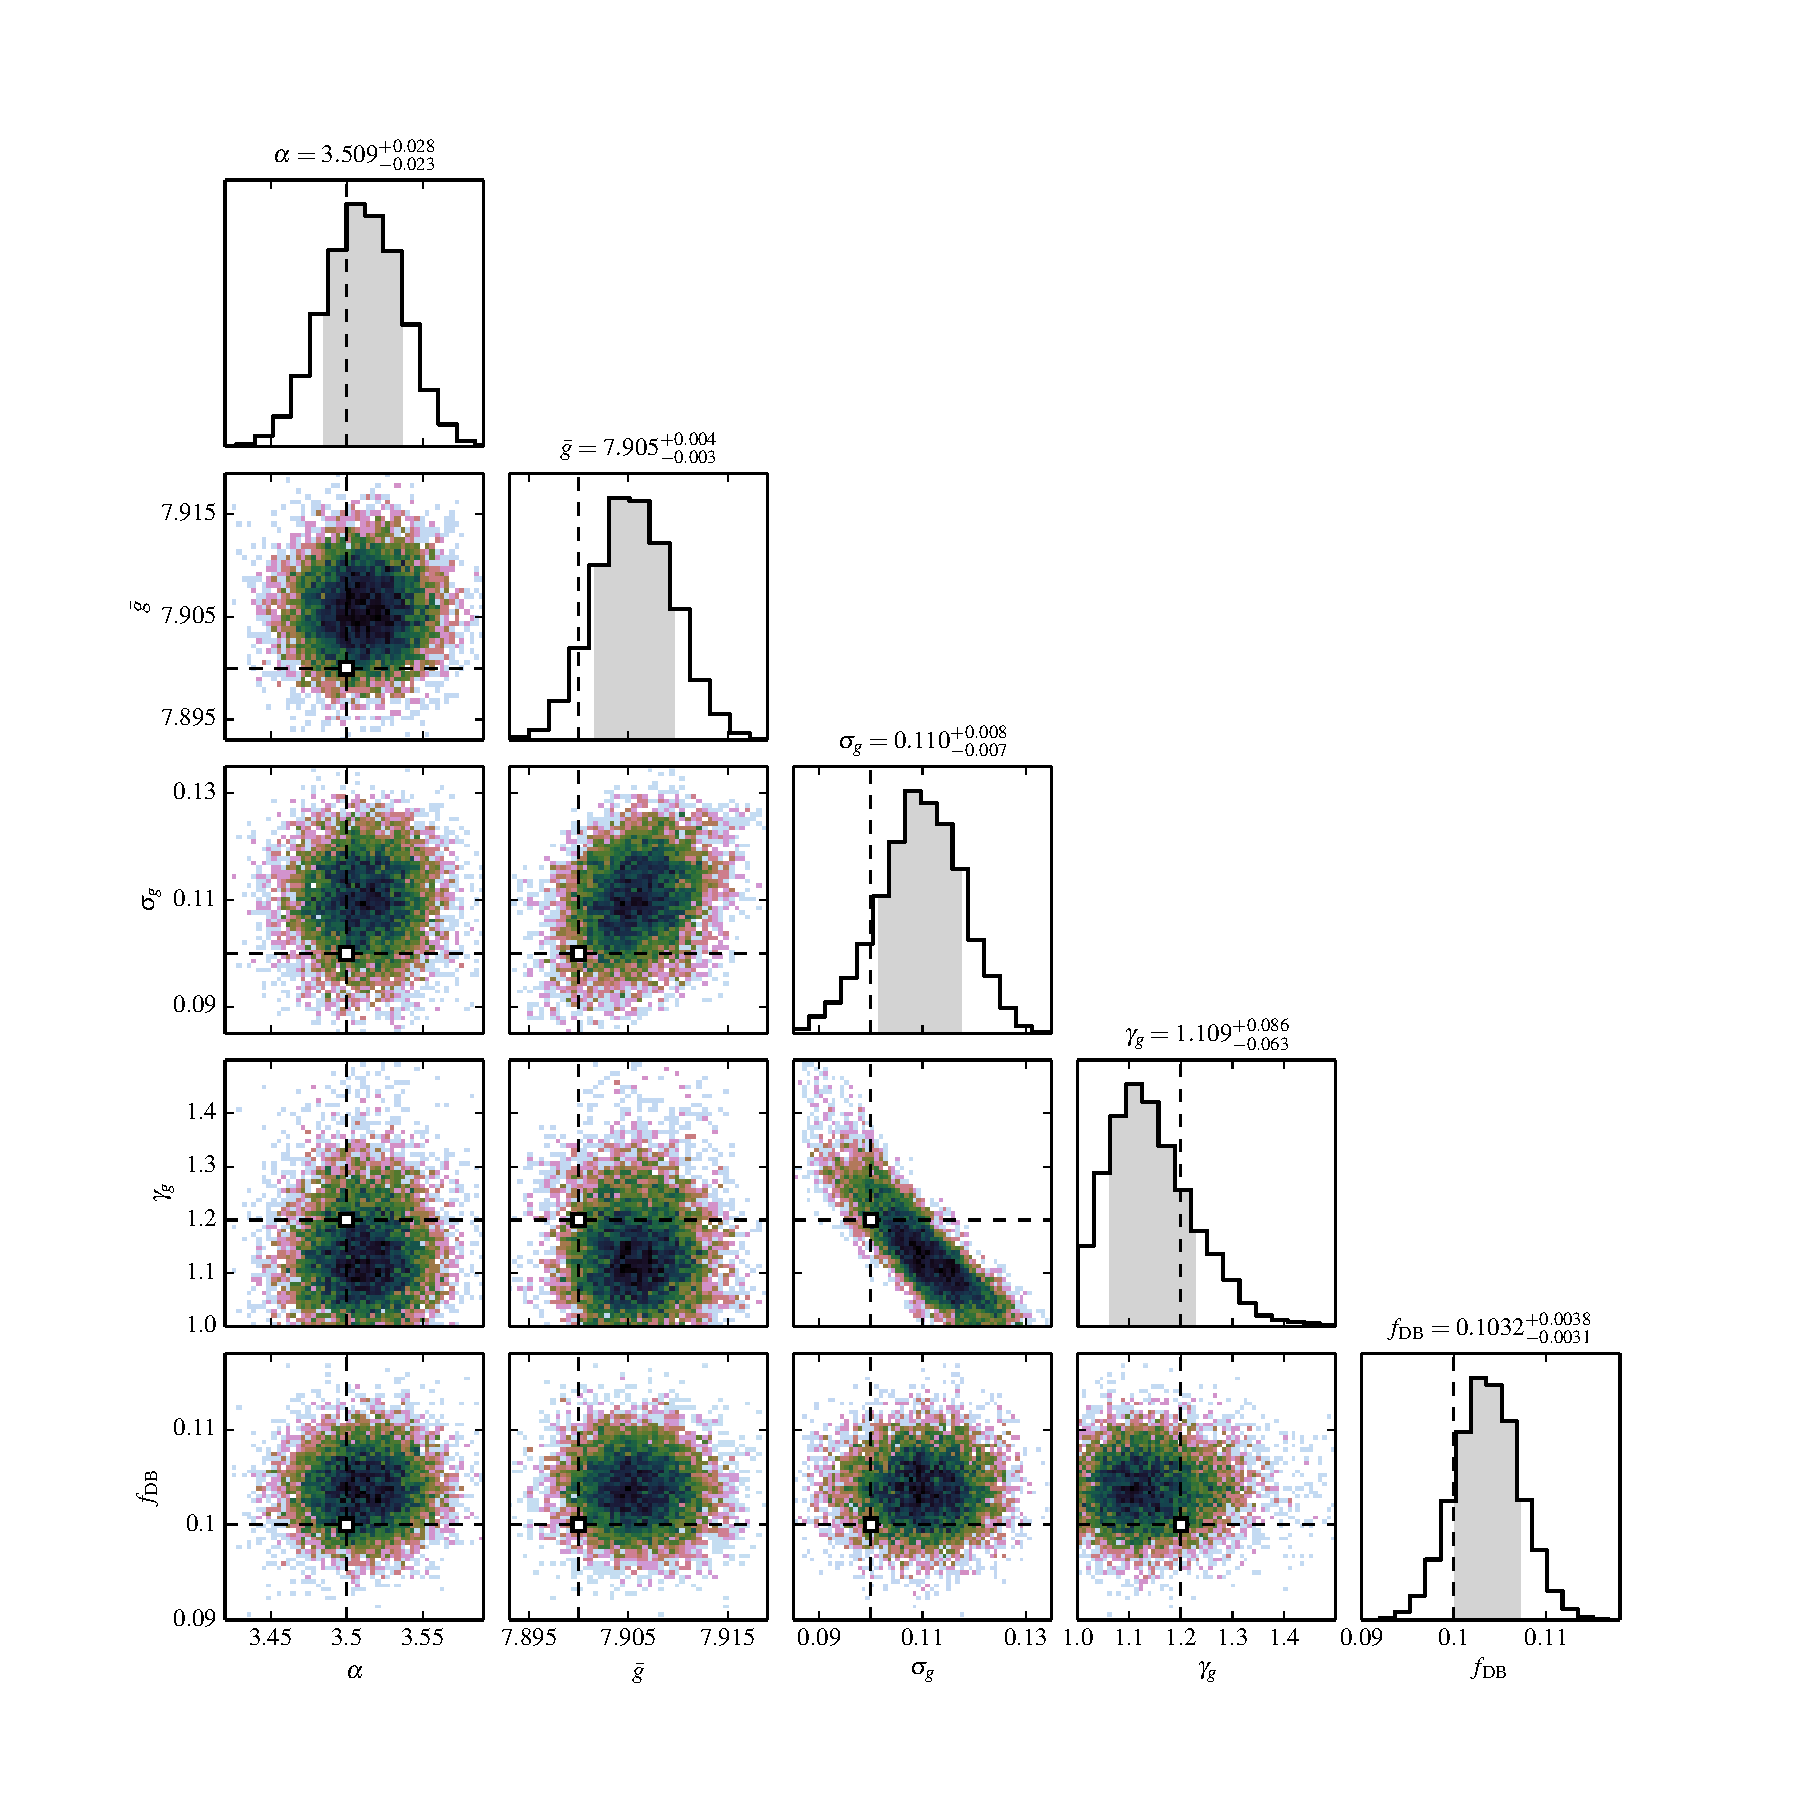
\includegraphics[width=1.\textwidth]{toy_chain.pdf}
    \caption{Posterior density of the population parameters, for a mock data set with no astrometric information.}
    \label{fig:chain}
\end{figure*}

\begin{figure*}
	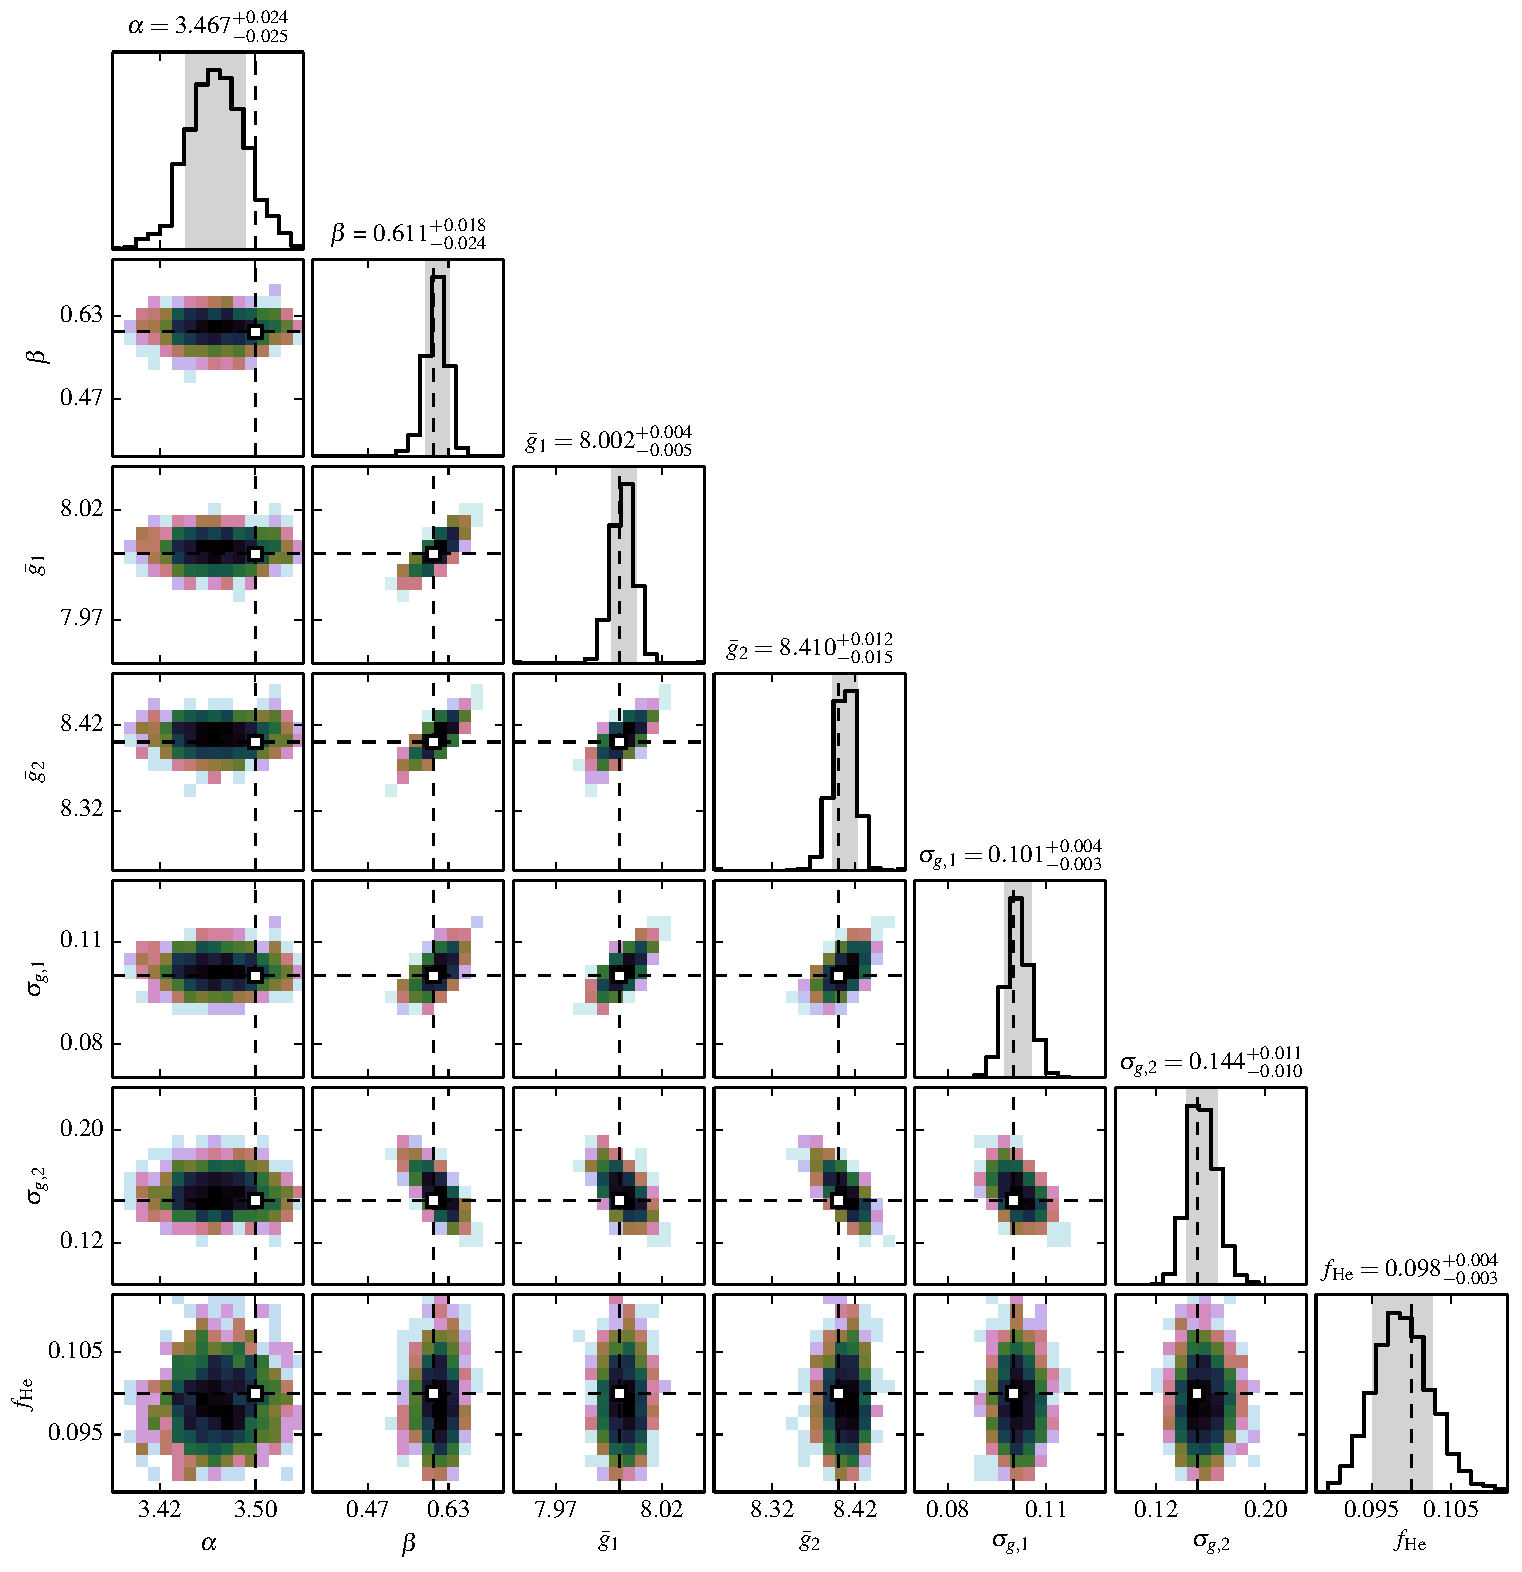
\includegraphics[width=1.\textwidth]{toy_chain_include-parallax.pdf}
    \caption{Posterior density of the population parameters, for a mock data set with parallax information.}
    \label{fig:chain_parallax}
\end{figure*}










\section{White dwarf subpopulations}

The actual population of white dwarfs in the Milky Way is of course much richer and complicated than the model described above. We only have white dwarfs of the hydrogen rich type (DA), while in reality there is something like 10 \% helium rich (DB) white dwarfs. Furthermore, younger white dwarfs are more abundant within the disk, while older white dwarfs have had more time to migrate into the halo.

In the case of several distinct populations, the total population is no longer described by a single set of population parameters $\popp$.






\subsection{DA and DB populations}

Hydrogen rich and helium rich white dwarfs, known as DA and DB, have different spectra and emission lines. This translates into somewhat different colors for DA and DB, such that they are differentiable from eachother with multiband photometry of sufficient precision. In order to account for both DA and DB populations, one can add the fraction of DB white dwarfs ($f_\text{DB}$) to the population paremeters $\popp$. In such a case we would add a labelling object parameter $X_i = \{\text{DA},\text{DB}\}$ to each object.

In the statistical model, as summarized in equation \eqref{eq:fullposterior}, we would replace the term

\begin{equation}
\begin{split}
	& \pr(\data_i | \objp_i) \pr(\objp_i | \popp)
	\rightarrow \\
	\Big[
	(1-f_\text{DB}) & \pr(\data_i | \objp_i,X_i=\text{DA}) \pr(\objp_i | \popp) + \\
	+ f_\text{DB} & \pr(\data_i | \objp_i,X_i=\text{DB}) \pr(\objp_i | \popp)
	\Big].
\end{split}
\end{equation}
Also the normalization term $\bar{N}$, as seen in equation \eqref{eq:normalization}, is changed by replacing

\begin{equation}
\begin{split}
	& S(\Teff,\logg,\mathbf{x}) \rightarrow \\
	\Big[
	 (1-f_\text{DB}) & S(\Teff,\logg,\mathbf{x},X=\text{DA})
	 + f_\text{DB} S(\Teff,\logg,\mathbf{x},X=\text{DB})
	 \Big].
\end{split}
\end{equation}






\subsection{Disk and halo populations}

It would be interesting to see qualitative differences between disk and halo white dwarfs. Do they have the same distribution of masses, same fraction of DA and DB stars, the same fraction of binary systems?

Each subpopulation would have its own set of population parameters, for example $\popp_\text{disk}$ and $\popp_\text{halo}$ for disk and halo white dwarfs. The spatial white dwarfs number density distributions would be different, so we would have $n_\text{disk}(\mathbf{x})$ and $n_\text{halo}(\mathbf{x})$. It would be necessary here to promote the number density (of some reference point, like at the Sun's position) to a population parameter, like $n_{0,\text{disk}}(\mathbf{x})$ and $n_{0,\text{halo}}(\mathbf{x})$, and include a Poisson total number count factor in the model.

Equation \eqref{eq:fullposterior} would instead read

\begin{equation}\label{eq:posterior_disk_halo}
\begin{split}
	\pr(\popp,\objp | \data ) = \\ \pr(\popp) \pr(N | \bar{N}) 
	\prod_i \frac{S(\data_i) \pr(\data_i | \objp_i) \Big[ \pr(\objp_i | \popp_\text{disk})+\pr(\objp_i | \popp_\text{halo}) \Big]}{\bar{N}(S,\popp_\text{disk},\popp_\text{halo})},
\end{split}
\end{equation}
where $\pr(N | \bar{N})$ is a Poisson number count likelihood. The total number count can be written as a sum of the number counts of the two subpopulations,

\begin{equation}
	\bar{N}(S,\popp_\text{disk},\popp_\text{halo})=\bar{N}_\text{disk}(S,\popp_\text{disk})+\bar{N}_\text{halo}(S,\popp_\text{halo}).
\end{equation}







\subsection{Binary population}

Binary white dwarf systems can be identified using only photometry and astrometry, in a similar way as what was used in \cite{2018ApJ...857..114W}. For a binary system, the likelihood is the same as is written in equation \eqref{eq:likelihood}, the difference being that the \emph{ugriz} apparent luminosities of the two component stars are added together, according to

\begin{equation}
	m_\text{sum} = - \frac{5}{2}\log_{10}\left( 10^{-\frac{5}{2}m_{A}}+10^{-\frac{5}{2}m_{B}}  \right),
\end{equation}
where $m_A$ and $m_B$ are the apparent magnitudes of the two component stars, in the relevant photometric band.

The posterior density of a binary will be written in terms of 5 parameters instead of 3, as we have temperature and surface gravity of two component stars (although at the same parallax, assuming a tight orbit).

We construct a population of mock binaries by random pairing of the singles population and the same selection criteria, although we also add a constraint in terms of cooling time of the two component stars. In addition to the effective temperature and surface gravity distributions of the two component stars, as described by equation \eqref{eq:T&g}, we also have an additional term

\begin{equation}\label{eq:time_difference}
	\exp\left(
	-\frac{[t_\text{cool}(\Teff_A,\logg_A)-t_\text{cool}(\Teff_B,\logg_B)]^2}{2\times (10^9~\text{yrs})^2}
	\right),
\end{equation}
where $t_\text{cool}(\Teff_{\{A,B\}},\logg_{\{A,B\}})$ is the cooling time of the respective component stars, as given by the Bergeron atmospheric model.

Figure \ref{fig:ROC_binaries} shows a receiver operator characteristic (ROC) curve for identification of binaries. The binaries are inferred with knowledge of the underlying population model. It is clear from the figure that most binaries can be very strongly identified, even with a zero false positive rate. The chosen time difference of $\sim 10^9$ years, set in equation \eqref{eq:time_difference}, prohibits the pairing of extremely cool and faint white dwarfs with hotter ones. The ROC curve is highly dependent on the allowed difference in cooling time. A stronger constraint on the difference in cooling time makes the component stars of more comparable brightness, and binaries are therefore easier to detect, and vice versa when a larger difference in cooling time is allowed.

\begin{figure}
	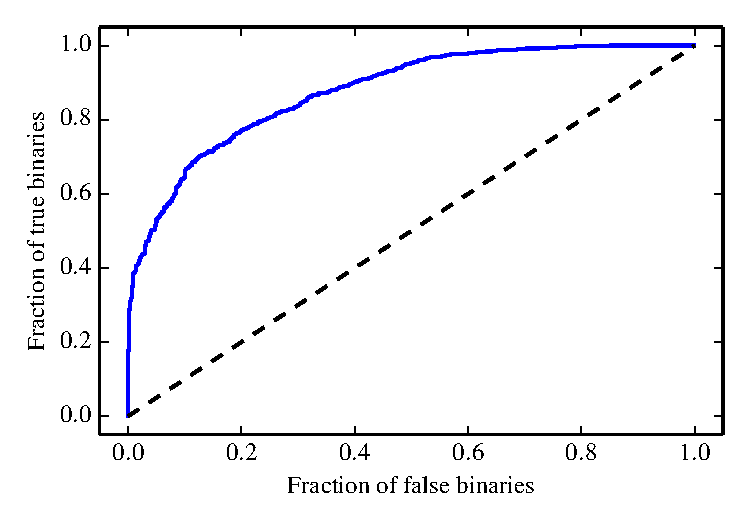
\includegraphics[width=\columnwidth]{ROC_binaries.pdf}
    \caption{A receiver operator characteristic (ROC) curve of binary identification, showing the rate of false positives versus true positives.}
    \label{fig:ROC_binaries}
\end{figure}

This identification is made on mock data when the underlying population model is known. Working with actual data comes with many complications, not least the fact that the population model is unknown and inferred. Even so, this test shows that it should be possible to detect and infer properties about white dwarf binary population. An important aspect that is not accounted for here is that white dwarf binaries are not drawn from the same distribution of masses as the population of single white dwarfs. A tight binary system goes through phases of mass transfer and shared envelopes; thus a white dwarf binary component is expected to have low mass and surface gravity. This would actually make binaries even easier to detect, as they are brighter due to multiplicity, and brighter still from being low mass and larger in size.







\section{Conclusions}








\section*{Acknowledgements}

The Acknowledgements section is not numbered. Here you can thank helpful
colleagues, acknowledge funding agencies, telescopes and facilities used etc.
Try to keep it short.

%%%%%%%%%%%%%%%%%%%%%%%%%%%%%%%%%%%%%%%%%%%%%%%%%%

%%%%%%%%%%%%%%%%%%%% REFERENCES %%%%%%%%%%%%%%%%%%

% The best way to enter references is to use BibTeX:

\bibliographystyle{mnras}
\bibliography{refs} % if your bibtex file is called example.bib

%%%%%%%%%%%%%%%%%%%%%%%%%%%%%%%%%%%%%%%%%%%%%%%%%%

%%%%%%%%%%%%%%%%% APPENDICES %%%%%%%%%%%%%%%%%%%%%

\appendix

\section{Some extra material}


%%%%%%%%%%%%%%%%%%%%%%%%%%%%%%%%%%%%%%%%%%%%%%%%%%


% Don't change these lines
\bsp	% typesetting comment
\label{lastpage}
\end{document}

% End of mnras_template.tex